
\chapter{First Order ODEs}

\noindent  
This chapter covers the following ideas. When you create your lesson plan, it should contain examples which illustrate these key ideas. Before you take the quiz on this unit, meet with another student out of class and teach each other from the examples on your lesson plan. 



\begin{enumerate}
\item Be able to interpret the basic vocabulary of differential equations. In particular, interpret the terms ordinary differential equation (ODE), initial value, initial value problem (IVP), general solution, and particular solution.
\item Use the three step modeling process (express, solve, and interpret) to analyze exponential growth and decay, Newton's law of cooling, mixing, and the logistics equation. 
\item Identify and solve separable ODES and exact differential forms. Use integrating factors and substitutions to solve additional ODEs.
\item Use Laplace transforms to solve first order ODEs.
\end{enumerate}




\section{Basic Concepts and Vocabulary}
A differential equation is an equation which involves derivatives (of any order) of some function.  For example, the equation $y^{\prime\prime}+xy^\prime+\sin(xy)=xy^2$ is a differential equation. An \textbf{ordinary differential equation (ODE)} is a differential equation involving a function $y(x)$ whose domain is one dimensional. A solution to an ODE on an interval $J=(a,b)$ is a function $y(x)$ defined on the interval $J$ which satisfies the ODE.  To verify that a function is a solution to an ODE, calculate derivatives and put them in the ODE. If the resulting equation is an identity for all $x\in J$, then you have a solution. The order of an ODE is the largest order derivative that appears in the ODE. 

Typically a solution to an ODE involves an arbitrary constant $C$. There is often an entire family of curves which satisfy a differential equation, and the constant $C$ just tells us which curve to pick. A \textbf{general solution} of an ODE is all possible solutions of the ODE.  A \textbf{particular solution} is one of infinitely many solutions of an ODE. Often an ODE comes with an \textbf{initial condition} $y(x_0)=y_0$ for some values $x_0$ and $y_0$. We can use these initial conditions to find a particular solution of the ODE. An ODE, together with an initial condition, is called an \textbf{initial value problem (IVP)}.  

\begin{example}
The ODE $y^\prime = ky$ has the general solution $y=ce^{kx}$ for $x\in(-\infty,\infty)$. We check that this is a solution by calculating $\frac{d}{dx}ce^{kx} = kce^{kx}=ky$. This is a first order ODE because only the first derivative and no higher derivatives appear in the ODE.  If the initial condition $y(0)=3$ were also in the problem, then the particular solution to this IVP is found by solving for $c$ in the equation $3=ce^{k0}$.  This simplifies to $c=3$, so $y(x) = 3e^{kx}$ is the solution to the IVP  $y^\prime = ky$, $y(0)=3$.
\end{example}

%\subsection{Direction Fields}
%A first order ODE of the form $y^\prime=f(x,y)$ can be used to describe a vector field which represents the slope of $y$ at each point in the plane. Since $y^\prime$ is the slope of $y$, the graph of the vector field $\vec F = \left<1,y^\prime\right>$ gives a picture of how $y$ changes depending on which point $(x,y)$ in the plane you are at.  This graph is called a direction field, and it is used to visually see what a solution should look like.  Solutions to a first order ODE will follow the direction vectors in the direction field.  Some ODEs are so complex that no known method of solving them is available, and so direction fields give a way of visually approximating a solution.  Some examples follow. The first two examples include several particular solutions of the ODE for different initial conditions.
%
%
%\newcommand{\mywidth}{1.3in}
%\begin{center}
%\begin{tabular}{cccc}
%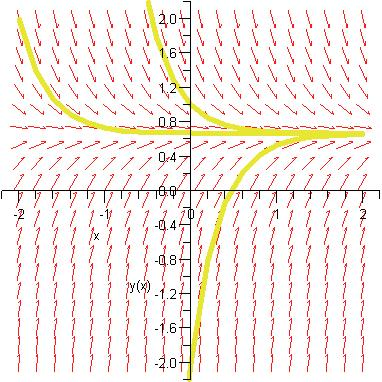
\includegraphics[width=\mywidth]{Basic-ODEs/dirfield-1}&
%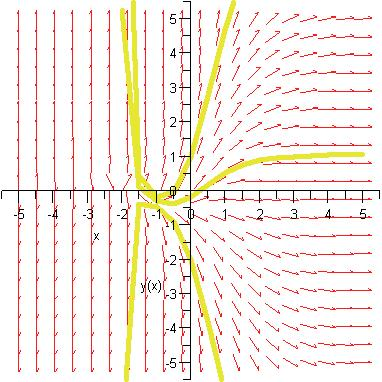
\includegraphics[width=\mywidth]{Basic-ODEs/dirfield-2}&
%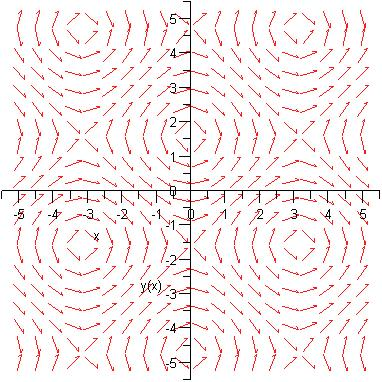
\includegraphics[width=\mywidth]{Basic-ODEs/dirfield-3}&
%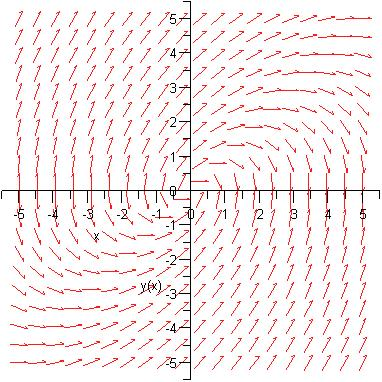
\includegraphics[width=\mywidth]{Basic-ODEs/dirfield-4}
%\\
%$y^\prime+3y = 2$&
%$e^{x}\frac{dy}{dx}= 2y+\cos(x)$ &
%$\cos(y)y^\prime= \sin(x)$ &
%$(x-y)dx+ydy=0$
%\end{tabular}
%\end{center}
%
% 




\section{Modeling Basics}
Many quantities in the world can be described in terms of rates of change. Differential equations arise in any physical model where rates of change are part of the model. Modeling requires that we (1) express quantities in terms of mathematical equations, (2) solve those equations, and (3) interpret the results in the context of our original problem.  The first and third steps require human intervention, while the second step can often be solved with the aid of technology. We will start by looking at three models: exponential growth and decay, Newton's law of cooling,  and mixing. I will illustrate steps (1) and (3) first, and then in the next section we will focus on methods of solving.


\subsection{Exponential Model}
Exponential growth and decay models radioactive decay, retirement investing, carbon dating, population growth, and more. The model is based on the principle that the rate of change of a quantity is directly proportional to the quantity itself.  The rate of decay of a radioactive isotope is proportional to the amount of the isotope that remains.  The rate of increase in a retirement investment is proportional to how much money is in the retirement investment. If you double an investment, then it should grow twice as quickly. We now follow the three steps.
\begin{enumerate}
	\item (Express) The derivative is proportional to the quantity itself can be expressed mathematically by the formula $y^\prime(x)=ky(x)$, where $k$ is some constant. 
	\item (Solve)  The general solution to this ODE is $y(x) = ce^{kx}$. (Solved in example~\ref{expsol})
	\item (Interpret) When $x=0$, we have $y=c$. This means that $c$ is the initial amount of a radioactive isotope, or the initial investment in a retirement portfolio.  The constant $k$ helps us determine how quickly an isotope decays ($k<0$), or how quickly an investment grows ($k>0$).  
\end{enumerate}





\subsection{Newton's Law of Cooling}
One version of Newton's law of cooling states that the rate of change of temperature $\frac{dT}{dt}$ of a body (which conducts heat well) is proportional to the difference between the current temperature $T(t)$ of the body and the temperature $T_A$ of the surrounding atmosphere (which is assumed to be constant).
\begin{enumerate}
	\item (Express) Newton's law of cooling can be expressed mathematically as $ \frac{dT}{dt} = k(T-T_A)$ for some constant $k$.  If $T>T_A$, then the temperature needs to drop, so we know $k<0$. If $T<T_A$, then the temperature needs to rise, so $k<0$ gives $k(T-T_A)>0$ as the product of two negatives. In all cases, the constant $k$ will hence be negative.
	\item (Solve)  The general solution to this ODE is $y = T_A+ce^{kt}$ (solved in Example~\ref{newtonsol}).
	\item (Interpret) When $t=0$, we have $T(0)=T_A+c$. This means that $c=T(0)-T_A$ is the initial difference in temperature.  Since $k$ is always negative, as $t\to\infty$ the temperature $T(t)$ approaches $T_A$, the temperature of the surrounding atmosphere.  
\end{enumerate}

\subsection{Mixing Model}
We will encounter mixing problems throughout the semester of the following type.  Suppose a 5000 gallon tank contains a solution of water which initially contains 200 lbs of salt. The tank has an inflow valve, and an outflow value.  Suppose 30 gallons of water (with 3 lbs of salt per gallon) are pumped into the tank each minute. The mixture is evenly spread throughout the entire tank by constant stirring.  At the same time, 30 gallons of the stirred mixture flow through the outflow valve each minute.  Find the amount of salt in the tank at time $t$.

%\begin{wrapfigure}{l}{0pt}
%	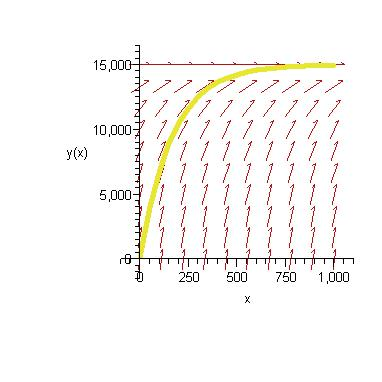
\includegraphics[width=1.5in]{Basic-ODEs/model-1}
%\end{wrapfigure}

\begin{enumerate}
	\item (Express) If we let $y(t)$ be the amount of salt in the tank at any time $t$, then $y^\prime=\text{(flow in)}-\text{(flow out)}$. The flow in is 
	$$\text{flow in }=\frac{30 \text{ gal}}{\text{min}}\bigg|\frac{3 \text{ lbs}}{\text{gal}} = \frac{90 \text{ lbs}}{\text{min}} \text{ of salt.}$$ 
The amount of salt lost per minute is proportional to the amount of salt in the tank. Since the tank holds 5000 gallons, and the outflow is 30 gal/min, we loose $\frac{30}{5000}$ of the water in the tank each minute.  Since the mixture is evenly stirred, this means that $\frac{30}{5000}$ of what currently is in the tank (which is $y$ lbs) should leave every minute.  So our flow out is\
	$$\text{flow out }=\frac{30 \frac{\text{gal}}{\text{min}}}{5000 \text{ gal}}\bigg|y \text{ lbs} = \frac{30}{5000}y \frac{\text{lbs}}{\text{min}} \text{ of salt.}$$ 
Hence $y^\prime = 90-\frac{30}{5000}y$. The initial condition is $y(0)=200$ lbs.
	\item (Solve) The general solution is $y(t) = 15000+c e^{(-3/500) t}$.  Using $y(0)=200$, we find $200=15000+c,$ or $c=-14800$.  So $y(t) = 15000-14800 e^{(-3/500) t}$.
	\item (Interpret) The salt content starts at 200 lbs and grows to a maximum of 15000 lbs as $t\to\infty$.  The quantity grows more rapidly at the beginning than at the end.
\end{enumerate}





\section{Basic Methods}
The modeling process often results in a differential equation. We will learn various methods of solving these differential equations. Software can solve the differential equations in this course,  however, the differential equations you may encounter in the future might not be solvable by any of the methods in this textbook or by software.  Understanding the ideas and processes which go into these methods will give you building blocks which you may need to creatively solve new differential equations.  

\subsection{Separable}
The most basic differential equation to solve is one in which you can ``separate'' the variables.  The idea is to rearrange the equation in the form $f(y)dy=g(x)dx$, where you separate the $x$ and $y$ terms so that they appear on different sides of the equation.  The solution is found by integrating each side.

\begin{example}[Exponential Model Solution] \label{expsol} Divide the differential equation $y^\prime = ky$ on both sides by $y$. Then multiply both sides by the differential $dx$ to obtain $\frac{1}{y}dy = k dx$. Integration on both sides yields $\ln|y| = kx+c$.  Exponentiating both sides gives $|y|=e^{kx+c}=e^{kx}e^c$. Now $e^c$ is a positive constant, so we rename that constant to be $c$ and obtain $|y|=ce^{kx}$ for $c>0$.  Removing the absolute values on $y$ allows $c$ to be any nonzero constant. If $c=0$, then the equation $y=0$ satisfies the differential equation $y^\prime = ky$, so we can let $c=0$ as well. This shows that a general solution to $y^\prime = ky$ is $y(x)=ce^{kx}$ for any constant $c$.
\end{example}

\begin{example}[Newton's Law of Cooling Solution] \label{newtonsol}The differential equation for Newton's law of cooling, $ \frac{dT}{dt} = k(T-T_A)$, is another separable ODE. Rearrange the equation as $\frac{1}{T-T_A}dT = kdt$.  Integration yields $\ln|T-T_A|=kt+c$.  Exponentiation gives $|T-T_A|=e^{kt+c}=e^{kt}e^c=ce^{kt}$.  Removing absolute values as before gives $T=T_A+ce^kt$ as a general solution. 
\end{example}

\subsection{Exact Differential Forms}
Recall that a vector field $\vec F=\left<M,N\right>$ is called a gradient field if there exists a function $f(x,y)$, called a potential for $F$, which satisfies $\nabla f = \vec F$. Recall also that $\vec F=\left<M,N\right>$ has a potential (under suitable conditions) if and only if $M_y=N_x$ (test for exactness). Similarly, a differential form $Mdx+Ndy$ is said to be exact if there exists a function $f(x,y)$ which satisfies $df=Df(x,y)\begin{bmatrix}dx\\ dy\end{bmatrix}= Mdx+Ndy$. If a first order differential equation can be written in the form $Mdx+Ndy=0$, and that differential form is exact, then a general solution to the ODE is $f(x,y)=c$ for any constant $c$, where $f$ is a potential for $\left<M,N\right>$. 
\marginpar{A general solution to $Mdx+Ndy=0$ is $f=c$ where $f$ is a potential for $\left<M,N\right>$ and $c$ is an arbitrary constant.}  
This is because the level curves of the potential ($f=c$) are orthogonal to the gradient of the potential, which is precisely what $\left<M,N\right>\cdot\left<dx,dy\right>=0$ means. 

\begin{example}
The differential equation $3xy^\prime = 2x-3y$ can be rewritten in the differential form $(3y-2x)dx+3xdy=0$. We calculate $M_y=\frac{\partial}{\partial y}(3y-2x) = 3$ and $N_x=\frac{\partial}{\partial x}(3x) = 3$. Since $M_y=N_x$, a potential exists. We integrate both terms and obtain  
$$\int M dx = 3xy-x^2 \quad\bigg|\quad \int N dy = 3xy.$$ Summing the integrals and ignoring duplicates, we obtain $f=3xy-x^2$ as a potential.  The general solution of $3xy^\prime = 2x-3y$ is $3xy-x^2=c$ for any constant $c$. We have written the solution implicitly (without solving explicitly for $y$). Solving for $y$ gives the explicit solution $y=\frac{c+x^2}{3x}$, however you may not always be able to solve for $y$.  
\end{example}

Notice that if a differential equation is separable $f(y)dy=g(x)dx$, then it represents an exact differential form, namely $-g(x)dx+f(y)dy=0$ has potential $-\int g(x)dx + \int f(y)dy$.  Every separable differential equation can be solved by considering exact differential forms. \marginpar{Solving an exact ODE is the BIG IDEA.} In fact, the goal of every method below is to rewrite the ODE so that it is an exact differential form, which means that finding a potential is the BIG IDEA of this unit.

\subsection{Integrating Factors (What to do if it isn't exact)}

Not every differential equation, when written in differential form $Mdx+Ndy=0$ is exact.  However, by multiplying both sides by an appropriate factor (called an integrating factor), often we can make the ODE exact. 

\begin{example}
The differential form $-kydx+dy=0$ (which models exponential growth) is not exact. However, if you multiply both sides by $e^{-kx}$, then the differential form $-ke^{-kx}ydx+e^{-kx}dy=0$ is exact with potential $f=ye^{-kx}$, and hence the solution is $ye^{-kx}=c$ or $y=ce^{kx}$ as before.  Alternatively, we could multiply both sides of $-kydx+dy=0$ by $\frac{1}{y}$. This gives the differential form $-kdx+\frac{1}{y}dy=0$, which is exact with potential $f=-kx+\ln|y|$. The general solution is thus $-kx+\ln|y|=c$ which becomes $\ln|y|=kx+c$ and simplifies to $y=ce^{kx}$ as before. In either case we multiplied a non exact differential form by a factor (called an integrating factor) to obtain an exact differential form.  
\end{example}

Essentially every method we look at for this unit can be solved by finding an appropriate integrating factor and then finding a potential to get the general solution. So how do we find an appropriate integrating factor? If a differential form $Mdx+Ndy$ is not exact, then we seek a function $F$ so that $FMdx+FNdy$ is exact.  To simplify our work, we will consider two cases: (1) $F$ is a function which depends on only $x$, or (2) $F$ is a function which depends on only $y$.  
\begin{enumerate}
	\item If $F=F(x)$, then for $FMdx+FNdy$ to be exact we must have $(FM)_y=(FN)_x$, which is equivalent to $FN_y = FM_x+F_xM$. Rearranging (separating $F$ from the other terms) gives $ \frac{1}{F}F_x = \frac{M_y-N_x}{N}$. Integrating both sides yields $ \ln|F| = \int\frac{M_y-N_x}{N}dx$.  Solving for $F$ gives $ F(x)=e^{\int\frac{M_y-N_x}{N}dx}$. The preceding formula will give us our integrating factor as long as  $ \frac{M_y-N_x}{N}$ depends only on $x$.
	\item If $F=F(y)$, then for $FMdx+FNdy$ to be exact we must have $(FM)_y=(FN)_x$, which is equivalent to $FM_y+F_yM = FN_x$. Rearranging gives $ \frac{1}{F}F_y = \frac{N_x-M_y}{M}$. Integrating both sides yields $ \ln|F| = \int\frac{N_x-M_y}{M}dx$, and solving for $F$ gives $ F(y)=e^{\int\frac{N_x-M_y}{M}dy}$. The preceding formula will give us our integrating factor as long as  $ \frac{N_x-M_y}{M}$ depends only on $y$.

\end{enumerate}
\begin{observation}
If  $\ds \frac{M_y-N_x}{N}$ depends on $x$, then $\ds e^{\int \frac{M_y-N_x}{N} dx}$ is an integrating factor. If $\ds\frac{N_x-M_y}{M}$ depends on $y$, then $\ds e^{\int \frac{N_x-M_y}{M} dy}$ is an integrating factor.
\end{observation}

\begin{example}
To solve the differential equation $(x+y)dx+3xdy=0$, we compute $M_y-N_x=1-3=-2$.  Division by $N$ gives $\frac{M_y-N_x}{N} = \frac{-2}{3x}$.  Hence $F=e^{\int -2/(3x) dx} = e^{-2/3 \ln(x)}=x^{-2/3}$. Then the differential form $(x^{1/3}+x^{-2/3}y)dx+3x^{1/3}dy=0$ has potential $\frac{3 x^{4/3}}{4}+3x^{1/3}y$.  So a general solution is $\frac{3 x^{4/3}}{4}+3x^{1/3}y=c$ or $y=\frac{c-\frac{3 x^{4/3}}{4}}{3x^{1/3}} $.
\end{example}

\subsection{Linear ODEs - a common special form}

A linear ODE is an ODE of the form $y^\prime+p(x)y=q(x)$. It is linear in $y$ and $y^\prime$. The linear ODE $y^\prime+p(x)y=0$ is separable, hence can be solved.  If $q(x)$ is not 0, we rewrite the linear ODE in differential form, getting $(p(x)y-q(x))dx+dy=0$. Since $\frac{M_y-N_x}{N} = (p(x)-1)/1=p(x)$ only depends on $x$, we use the integrating factor $F(x)=e^{\int p dx}$ to solve the differential equation. 

\begin{example}
To solve $y^\prime +2xy =3x$, we multiply by the integrating factor $F(x) = e^{\int 2x dx}= e^{x^2}$, and obtain $(2xye^{x^2}-3xe^{x^2})dx+e^{x^2}dy=0$. A potential is $u=ye^{x^2}-\frac32 e^{x^2}$, so the general solution is $ye^{x^2}-\frac32 e^{x^2}=c$, or $y=ce^{-x^2}+\frac32$. 
\end{example}

\subsection{$u$-Substitutions (How to make it exact)}
If an appropriate integrating factor cannot be found to make an ODE exact, then sometimes a substitution will get the job done.  Which substitution to make may require ingenuity.  However, sometimes the appropriate substitution to make can be seen by examining the function itself to see if there are complex parts which could be simplified by a substitution.  We will illustrate this approach with three common substitutions. This process is very similar to $u$-substitution from first semester calculus. 


\subsubsection{Homogeneous ODEs, $u=y/x$}
Some ODE's can be reduced to separable form by using the substitution $u=y/x$. If an ODE of the form $y^\prime = f(x,y)$ satisfies $y^prime=f(tx,ty)$ (replacing each $x$ and $y$ with $tx$ or $ty$ does nothing), then we call the ODE a homogeneous first order ODE. In such cases, the substitution $u=y/x$ will reduce the ODE to separable form. If an ODE has $y/x$ terms or $x/y$ terms in it, try this kind of substitution. We substitute $y=ux$ and $y^\prime = xu^\prime+u$ and then try to separate variables or find an integrating factor. Rather than memorizing these equations, it is easiest to just carry out the computations each time.

\begin{example}
The differential equation $4xy y^\prime = x^2+y^2$ is equivalent to $4y^\prime=\frac{x}{y}+\frac{y}{x}$. Replacing each $y$ with $ux$, and $y'$ with $xu'+u$, we obtain $4xu^\prime+4u = \frac{1}{u}+u$. This is equivalent to $4xu^\prime = \frac{1}{u}-3u=\frac{1-3u^2}{u}$.  Separating variables we obtain $\frac{4u}{1-3u^2}u^\prime = \frac{1}{x}$. Integration on both sides yields $\ds \frac{4}{-6}\ln|1-3u^2| = \ln|x|+c$. Exponentiating both sides eliminates the absolute values and gives the equation $(1-3u^2)^{-2/3} = cx$ (this $c$ is different than the first). Now substitute back in $u=y/x$ and solve for $y$, to obtain $1-3(y/x)^2 = cx^{-3/2}$, or $y=\pm x\sqrt{1/3- cx^{-3/2}}=\pm 1/3\sqrt{3x^2- c\sqrt{x}}$ (again $c$ has changed) as a solution for any constant $c$. 
\end{example}

\subsubsection{Bernoulli Equations, $u=y^{1-n}$}
A Bernoulli equation is an ODE of the form $y^\prime+p(x)y=r(x)y^n$. To solve such an ODE, let $u=y^{1-n}$. This means $u^\prime = (1-n)y^{-n}y^\prime = (1-n)y^{-n}(ry^n-py) = (1-n)(r-py^{1-n}) = (1-n)(r-pu)$.  By using this transformation, the ODE become a linear ODE of the form $u^\prime +(1-n)p(x)u=(1-n)r(x)$. Hence it has an integrating factor and can be solved as before. Again, it is easiest to carry out the computation with each example, rather than learn this general formula. 

\begin{example}
We'll solve the equation $y^\prime+y=3y^2$. First the substitution $u=y^{1-2}=y^{-1}$ gives $u^\prime = (-1)y^{-2}y^\prime = (-1)y^{-2}(3y^2-y) = (-1)(3-y^{-1}) = (-1)(3-u)$. So we have the linear ODE $u^\prime-u=-3$, which in differential form becomes $(3-u)dx+du=0$.  We compute $(M_u-N_x)/N=-1$, and so our integrating factor is $F(x)=e^{-x}$. The differential form   $(3e^{-x}-ue^{-x})dx+e^{-x}du$ is exact and has potential $f=-3e^{-x}+ue^{-x}$. Hence a solution is written implicitly as $-3e^{-x}+\frac{1}{y}e^{-x}=c$ or explicitly as $y=\frac{e^{-x}}{c+3e^{-x}} = \frac{1}{ce^x+3}$.
\end{example}


\subsubsection{Logistic Equation - A Bernoulli Model}
The logistic equation is $\frac{dy}{dt}=Ay-By^2$. It is used to model population growth, spread of disease, and other quantities which have an upper bound. If $B=0$, then we obtain the exponential model which we can already solve. This type of growth occurs with small populations where there is plenty of space to grow.  The term $-By^2$ is added to the model to prevent overgrowth, and places a population maximum on the model.  To solve the logistic equation, we let $u=y^{1-2}=y^{-1}$ as the equation is a Bernoulli equation. Differentiating gives $u^\prime=-y^{-2}y^\prime = -y^{-2}(Ay-By^2) = -(Ay^{-1}-B) = B-Au$, or $(Au-B)dx+du=0$.  Since $(M_u-N_x)/N=A$, we multiply by the integrating factor $F(x)=e^{\int Adx}=e^{Ax}$. The exact differential form $(Aue^{Ax}-Be^{Ax})dx+e^{Ax}du$ has potential $ue^{Ax}-\frac{B}{A}e^{Ax}$, so a general solution is $ue^{Ax}-\frac{B}{A}e^{Ax}=c$, or $\frac{1}{y}e^{Ax}-\frac{B}{A}e^{Ax}=c$. Solving for $y$ gives $y=\frac{e^{Ax}}{c+B/A e^{Ax}} = \frac{1}{ce^{-Ax}+B/A}$. Alternatively, we can multiply everything by $A$ to write $y=\frac{A}{ce^{-Ax}+B}$ 

\begin{example}
Let's solve the logistics equation $\frac{dy}{dt}=4y-y^2$. 
We let $u=y^{1-2}=y^{-1}$ as the equation is a Bernoulli equation. Differentiating gives $u^\prime=-y^{-2}y^\prime = -y^{-2}(4y-y^2) = -(4y^{-1}-1) = 1-4u$, or $(4u-1)dx+du=0$.  Since $(M_u-N_x)/N=4$, we multiply by the integrating factor $F(x)=e^{\int 4dx}=e^{4x}$. The exact differential form $(4ue^{4x}-e^{4x})dx+e^{4x}du$ has potential $ue^{4x}-\frac{1}{4}e^{4x}$, so a general solution is $ue^{4x}-\frac{1}{4}e^{4x}=c$, or $\frac{1}{y}e^{4x}-\frac{1}{4}e^{4x}=c$. Solving for $y$ gives $y=\frac{e^{4x}}{c+1/4 e^{4x}}$ or $y = \frac{4}{ce^{-4x}+1}$ (where $c$ was changed at the last step). 

\end{example}










\section{Finding Laplace Transforms and Inverses}
Recall that the Laplace transform of a function $f(t)$ defined for $t\geq 0$ is $F(s)=L(f(t))=\int_0^\infty e^{-st}f(t)dt$. The function $f(t)$ is called the inverse Laplace transform of $F(s)$, and we write $f(t)=L^{-1}(F(s))$. As a notational convenience, we use lower case letters and $t$ to describe original functions, and the same capital letter and $s$ to represent the Laplace transform.

\subsection{Finding the Laplace Transform - Review}
Let's start with a couple warm up examples. Remember that the improper integral computed with the Laplace transform will normally exist only for certain values of $s$. 
\begin{example}
If $f(t)=1$, then $F(s)=\int_0^\infty e^{-st}1dt= \frac{e^{-st}}{-s}\big|_0^\infty = \frac{1}{s}$, where the integral converges provided $s>0$. 
\end{example}
\begin{example}
If $f(t)=e^{at}$, then $F(s)=\int_0^\infty e^{-st}e^{at}dt=\int_0^\infty e^{-(s-a)t}dt= \frac{e^{-(s-a)t}}{-(s-a)}\big|_0^\infty = \frac{1}{s-a}$, where the integral converges provided $s>a$. 
\end{example}

Since integration can be done term by term, we have $L(af+bg)=aL(f)+bL(g)$ for functions $f,g$ and constants $a,b$.  We can use this to find many other Laplace transforms without having to do any more integration. 
\begin{example}
We have $L(\cosh a t) = \frac{1}{2}L(e^{at}+L(e^{-a t}))=\frac{1}{2}\left(\frac{1}{s-a}+\frac{1}{s+a}\right) = \frac{s}{s^2-a^2}$. Similarly $L(\sinh a t) = \frac{a}{s^2-a^2}$.  
\end{example}

The Laplace transform of the trigonometric functions $\cos x$ and $\sin x$ requires a little more work. The solution is similar to the transforms of $\cosh x$ and $\sinh x$, the only difference being a plus or minus in the denominator. Integration by parts twice yields $L(\cos \omega t) = \frac{s}{s^2+\omega^2}$ and $L(\sin \omega t) = \frac{\omega}{s^2+\omega^2}$.  
\begin{example} 
Let's find the transform of $\cos x$. We start by writing the definition of the transform $L(\cos \omega t) = \int_0^\infty e^{-st}\cos \omega t dt$.  The tabular method (illustrated on the side),
\marginpar{{\begin{tabular}{cc|c}
&$D$&$I$\\\hline
$+$&$\cos \omega t$&$e^{-st}$\\
$-$&$-\omega \sin \omega t$&$e^{-st}/(-s)$\\
$+$&$-\omega^2 \cos \omega t$&$e^{-st}/s^2$
\end{tabular}
}} 
after 2 iterations, gives 
\begin{align*}
\int_0^\infty &e^{-st}\cos \omega t dt \\
&= \left(\cos \omega t e^{-st}/(-s) +\omega \sin \omega te^{-st}/s^2\right)\big|_0^\infty - \int_0^\infty \omega^2 \cos \omega te^{-st}/s^2dt \\
&= 1/s - \omega^2/s^2 \int_0^\infty e^{-st}\cos \omega t dt.
\end{align*}
Replacing each integral above with $L(\cos \omega t)$ gives $$L(\cos \omega t) = 1/s-\omega^2/s^2L(\cos \omega t).$$
We have written the original integral in terms of itself. To simplify we combine like terms $(1+\omega^2/s^2)L(\cos \omega t) = \frac{1}{s}$, or $(s^2+\omega^2) L(\cos \omega t)=s$, and then we solve for the transform $L(\cos \omega t)=\frac{s}{s^2+\omega^2}$. The computation of $L(\sin x)$ is very similar, but results with an $\omega$ in the numerator instead of $s$.
\end{example}

Integration by parts also shows that $L(t^n) = \frac{n!}{s^{n+1}}$ for integers $n$. 
For convenience, table \ref{laplacetable} summarizes the Laplace Transforms we will use most often. Feel free to use this table as you find Laplace transforms and their inverses.  With practice, you will memorize this table.
\begin{table}
\begin{center}
\begin{tabular}[t]{|c|cc|}
\hline
$f(t)$ & $F(s)$ & provided\\
\hline\hline
$1$					&$\dfrac{1}{s}$ 							&$s>0$\\\hline
$t^n$				&$\dfrac{n!}{s^{n+1}}$ 			&$s>0$\\\hline
$e^{at}$		&$\dfrac{1}{s-a}$ 			&$s>a$\\\hline
$f'$					&$sL(f)-f(0)$ 						&\\\hline
\end{tabular}
\quad
\begin{tabular}[t]{|c|cc|}
\hline
$f(t)$ & $F(s)$ & provided\\
\hline\hline
$\cos(wt)$  &$\dfrac{s}{s^2+\omega^2}$ 			&$s>0$\\\hline
$\sin(wt)$  &$\dfrac{\omega}{s^2+\omega^2}$ 			&$s>0$\\\hline
$\cosh(wt)$ &$\dfrac{s}{s^2-\omega^2}$ 			&$s>|\omega|$\\\hline
$\sinh(wt)$ &$\dfrac{\omega}{s^2-\omega^2}$ 			&$s>|\omega|$\\\hline
\end{tabular}

\caption{Table of Laplace Transforms}
\label{laplacetable}
\end{center}
\end{table}


\subsection{Finding an Inverse Laplace Transform}
If the Laplace transforms of two functions are the same, then the two functions must be the same. This fact allows us to invert the Laplace transform and obtain the only function with a given Laplace transform.  Inverting a Laplace transform often involves matching the transformed function up with a function from a table, and then using the table to invert the transform.  We'll illustrate this with a few examples.

\begin{example}
To find the inverse Laplace transform of $F(s) = \dfrac{7}{s^3}$, first notice that $\dfrac{2}{s^3}$ is the transform of $t^2$. We rewrite $F(s) = \dfrac{7}{s^3} = \dfrac{7}{2}\dfrac{2!}{s^3}$, and then find the inverse transform as $L^{-1}(F(s)) = \dfrac{7}{2}t^2$.
\end{example}

\begin{example}
To find the inverse Laplace transform of $\ds F(s) = \frac{3s+4}{s^2+25}$, we notice that the transforms of $\cos(5t)$ and $\sin(5t)$ are $s/(s^2+5^2)$ and $5/(s^2+5^2)$.  We rewrite $$F(s)  = \frac{3s+4}{s^2+25}= 3\frac{s}{s^2+25} +\frac{4}{5} \frac{5}{s^2+25},$$ and then the inverse transform is $3\cos(5t)+\dfrac{4}{5}\sin(5t)$.
\end{example}

\begin{example}
To find the inverse Laplace transform of $F(s) = \dfrac{3s+1}{s^2+3s+2}$, we start by factoring the denominator as $(s^2+3s+2) = (s+2)(s+1)$.  We then use a partial fraction decomposition to write $$\dfrac{3s+1}{s^2+3s+2} = \dfrac{A}{s+2}+\dfrac{B}{s+1}.$$ Multiplication on both sides by $s^2+3s+2$ gives $$(3)s+(1) = A(s+1)+B(s+2) = (A+B)s+(A+2B).$$  Since the left and right sides are both linear equations of $s$, the coefficients must be equal so we must have $3=A+B$ and $1=A+2B$. The solution is $B=-2$ and $A=5$.  This means that $\ds F(s) = 5\frac{1}{s+2}-2\frac{1}{s+1}$, which means the Laplace inverse is $f(t) = 5e^{-2t}-2e^{-t}$.
\end{example}


\section{Solving IVPs}

\subsection{The Transform of a derivative}
The Laplace transform of a derivative is, using integration by parts, $$L(f^\prime)=\int_0^\infty e^{-st}f^\prime (t)dt = (e^{-st}f(t))\big|_0^\infty + s\int_0^\infty e^{-st}f (t)dt  = sL(f)-f(0).$$  We can use this formula to solve ODEs.

Here's the big idea. Given an ODE, take the Laplace transform of each side, giving what is called the subsidiary equation.  This equation can be solved for $L(y)=Y(s)$ using only algebra.  You then compute $L^{-1}(Y(s))$ to find the solution to the IVP $y(t)$.  This may involve finding a partial fraction decomposition. Laplace transforms reduce many IVPs to a 3 step process (1) convert to the subsidiary equation, (2) use algebra to solve for $Y$, performing a partial fraction decomposition if needed, (3) find inverse Laplace transform.

The following two examples represent the basic ideas used to solve pretty much every Laplace transform problem. We will be revisiting this idea throughout the semester.

\begin{example}
To solve the IVP $y^\prime +2y =0, y(0)=1$ we start by taking the Laplace transform of each side. This gives the subsidiary equation $sL(y)-y(0)+2L(y) = 0$, or using the notation $L(y)=Y$, we have $sY-1+2Y=0$.  Solving for $Y$ gives the equation $Y=\frac{1}{s+2}$. The inverse Laplace transform of both sides gives $y(t) = e^{-2t}$.  
\end{example}

\begin{example}
To solve the IVP $\ds y^\prime +2y =3, y(0)=1$, take the Laplace transform of each side. This gives the subsidiary equation $\ds sY-1+2Y=\frac{3}{s}$.  Solving for $Y$ gives the equation $\ds Y=\frac{s+3}{s(s+2)}$. The partial fraction decomposition $\ds \frac{s+3}{s(s+2)}=\frac{A}{s}+\frac{B}{s+2}$ requires we solve $\ds s+3 = A(s+2)+Bs$, or $1=A+B, 3=2A$ giving  $A=3/2$ and $B=-1/2$. Our subsidiary equation is now $\ds Y = \frac{3}{2}\frac{1}{s}-\frac{1}{2}\frac{1}{s+2}$. The inverse Laplace transform of both sides gives $\ds y(t) = \frac{3}{2}-\frac{1}{2}e^{-2t}$. 
\end{example}




